\chapter{Electron-Ion Collider}\label{cha:EIC} % chktex 24

The Electron-Ion Collider (EIC) is a planned accelerator facility to be built at Brookhaven National Laboratory [cite BNL] in the place of today's Relativistic Heavy Ion Collider (known as RHIC). Contrary to RHIC, which was built as an ion-ion collider, EIC will open new possibilities of probing the structure of nucleons by colliding the more complicated ions  with the comparably "simple-structured" electrons. Its versatile design will allow for the usage of a wide range of these ions – from protons (hydrogen ions) up to uranium nuclei [cite Silvia DIS].

\section{From RHIC to EIC}
For more than twenty years, RHIC has been instrumental for nuclear and particle physics. When it was commissioned in the year 2000, it became the first heavy ion collider capable of "smashing together" ions beyond the mass of a proton. These collisions, and the high energies at which they happened, allowed it to mimic the hot and dense conditions of the early universe. RHIC was also the first collider to utilize a spin-polarized beam of protons. The legacy of inovation will continue with the EIC, now also with the polarisation of the electron beam. [cite RHIC-facts]

The legacy of RHIC will also go on in the infrastructure, which will be partially reused for the EIC. Apart from the tunnels, the whole Yellow Ring of RHIC will be repurposed as the Hadron Storage Ring, with a small part of the Blue Ring used for a 41 GeV bypass. [cite Nagaitsev]. This is captured schematically in Figure~\ref{fig:eic:comparison}. On the other hand, due to the fact that the EIC will collide electrons, a separate electron accelerator will be built outside the original RHIC tunnel.
\\\,\\
Nejaké aktuálne informácie o urýchľovači?

\begin{figure}[H]
    \begin{subfigure}{0.4\linewidth}
        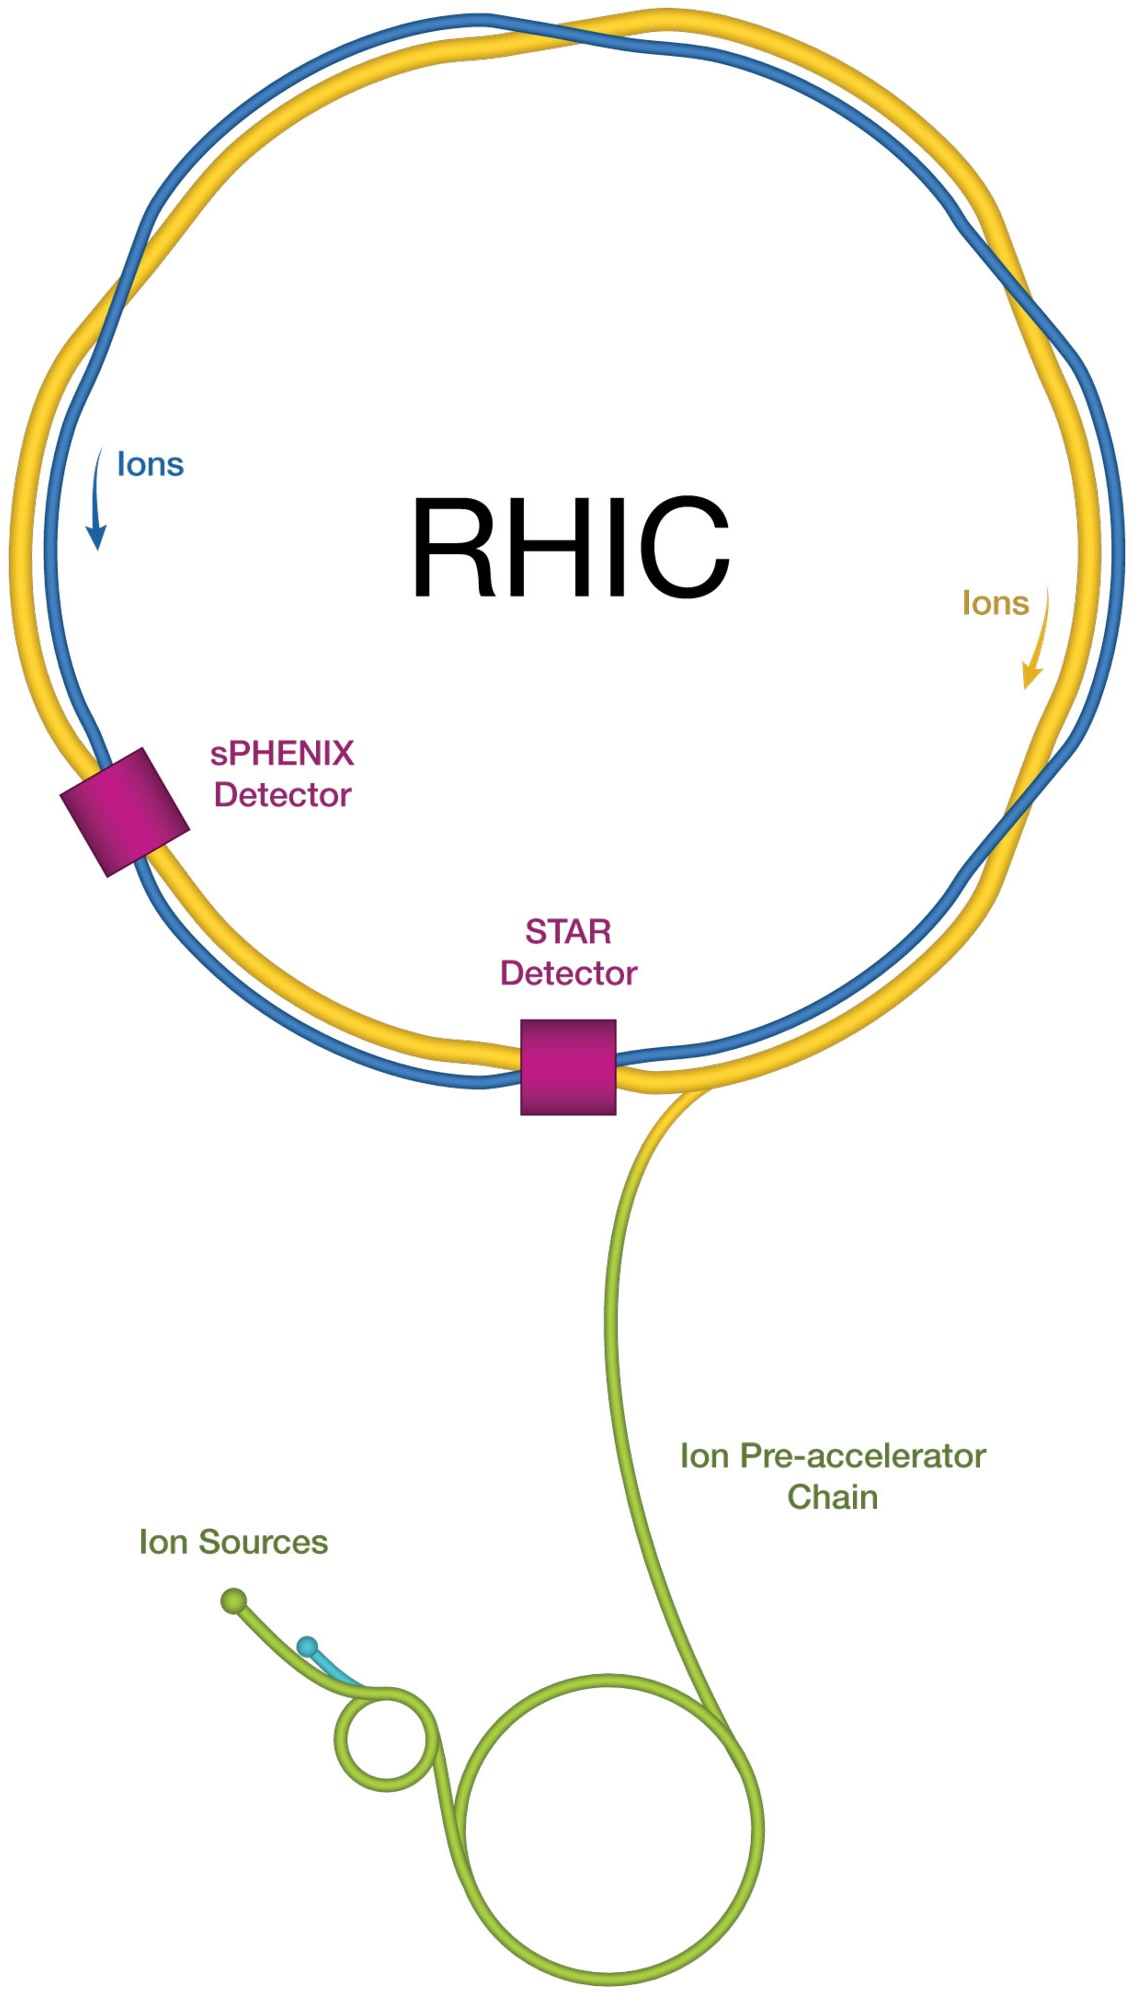
\includegraphics[height=10.4cm]{img/rhic.jpg}
        \caption{[cite RHIC image]}
        \label{fig:eic:comparison::rhic}
    \end{subfigure}
    %\hspace{0.02\linewidth}
    \raisebox{20\height}{\Huge$\rightarrow$}
    %\hspace{0.02\linewidth}
    \begin{subfigure}{0.52\linewidth}
        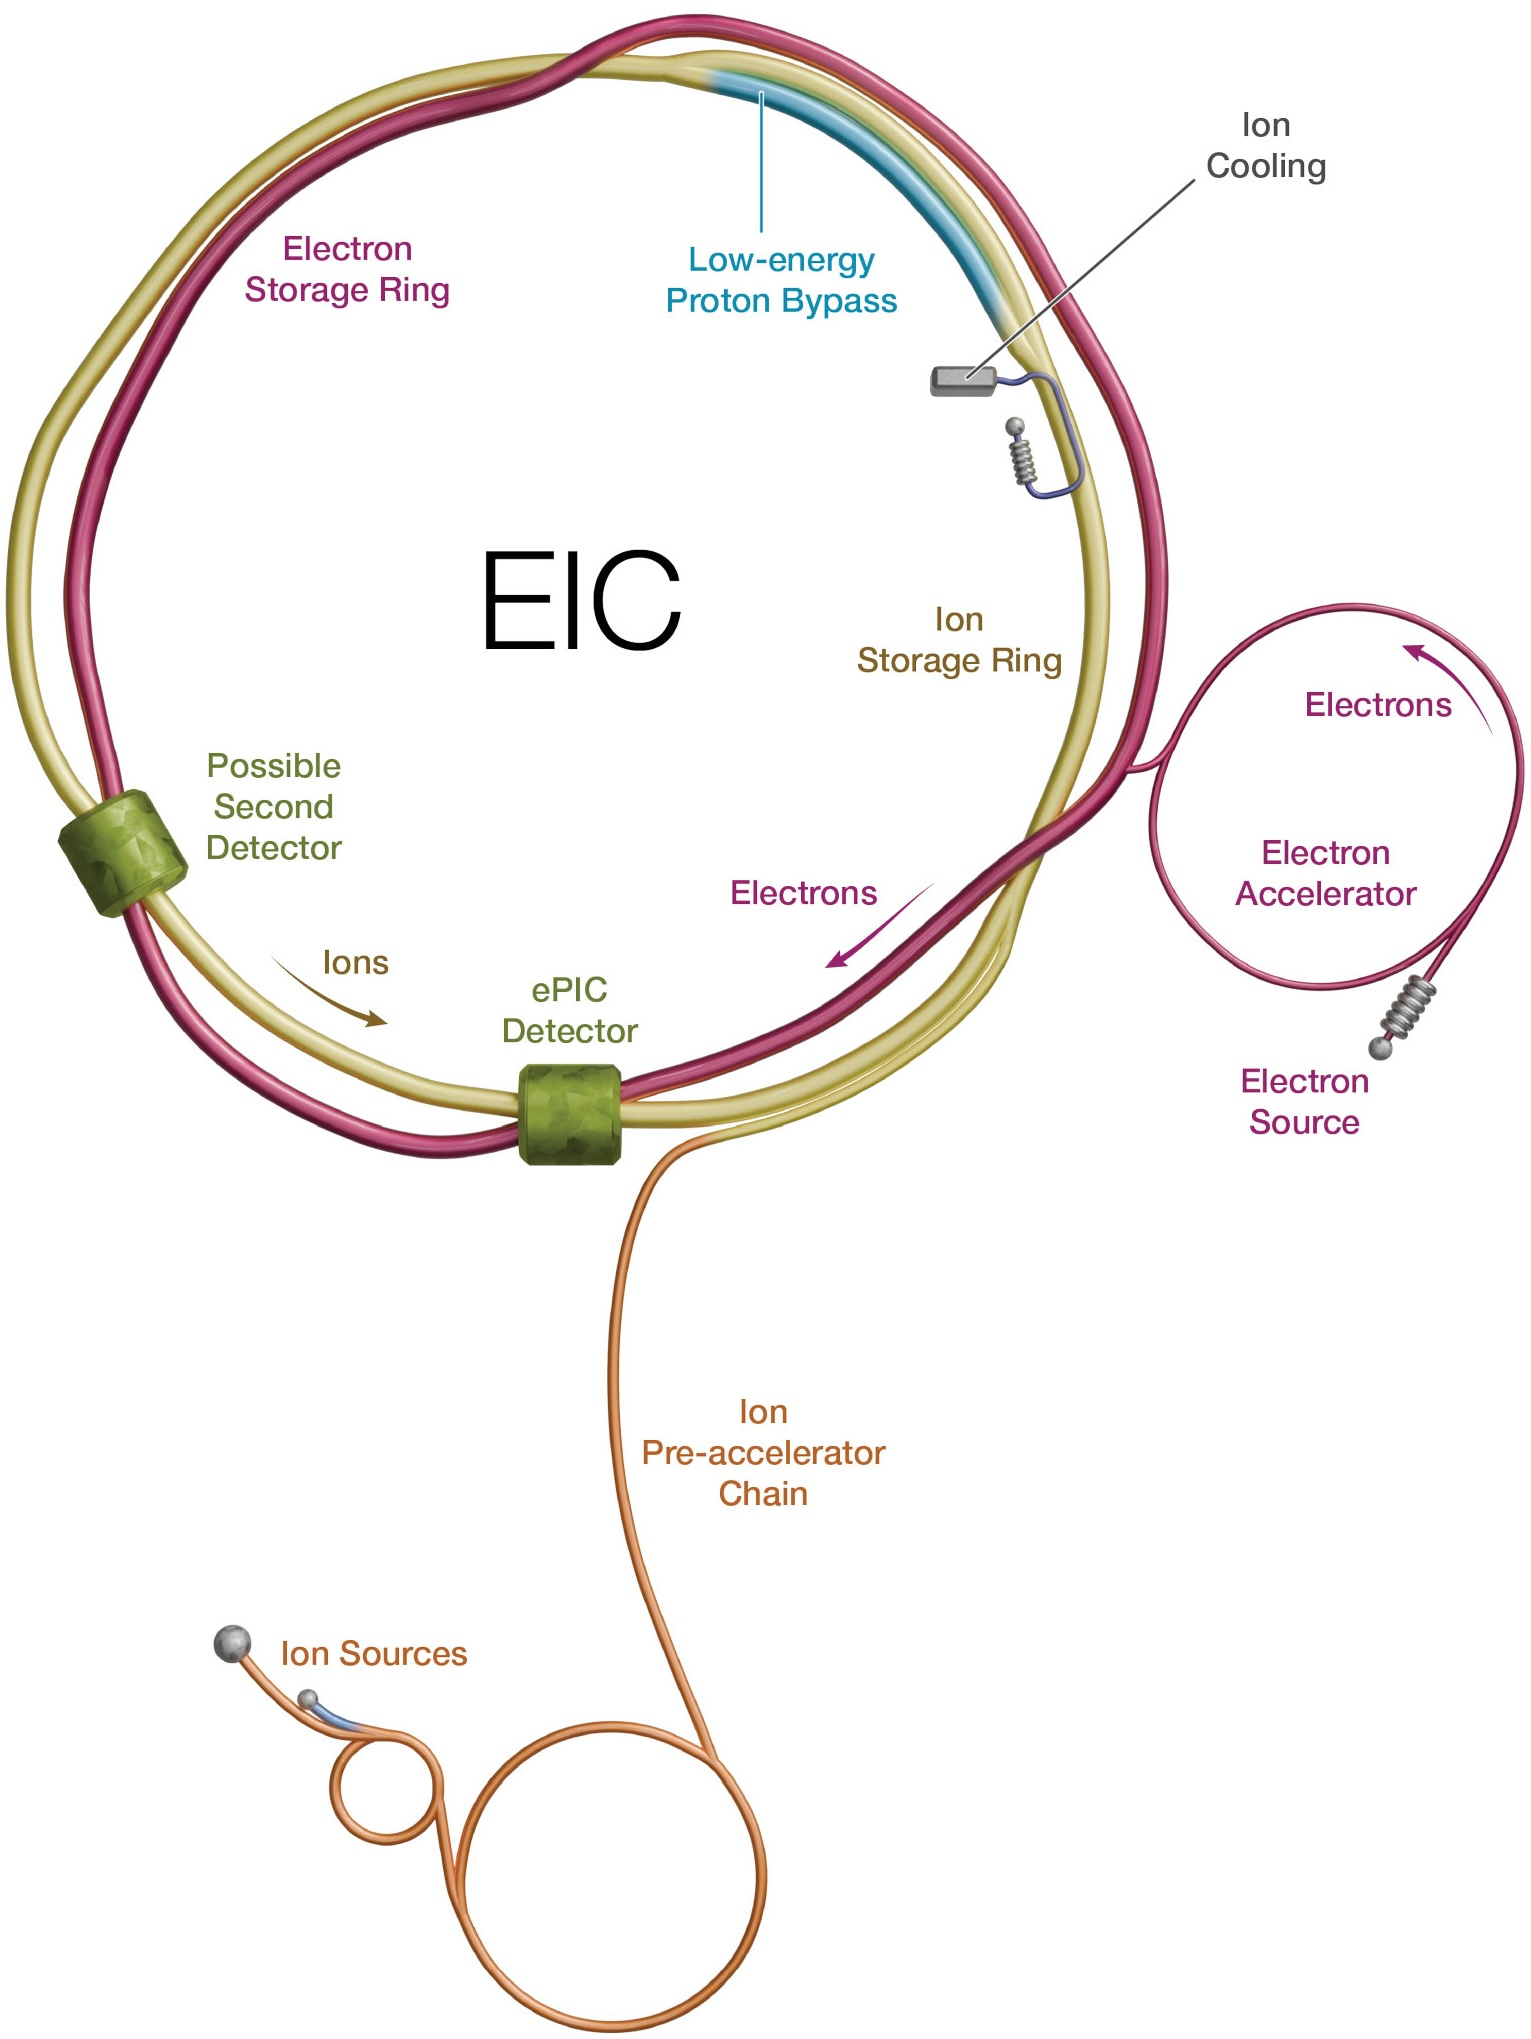
\includegraphics[height=10.4cm]{img/eic.jpg}
        \caption{[cite EIC image]}
        \label{fig:eic:comparison::eic}
    \end{subfigure}
    \caption{(a) Layout of the existing RHIC facility. (b) Conceptual design of EIC.}
    \label{fig:eic:comparison}
\end{figure}


% \section{Current Design Plan}

% \textit{the changes from usual illustrations (copied)}:\\
% In 2024, the project made several key EIC design decisions. They will lead to
% formal Project Scope changes after the Technical Change Control Board (TCCB)
% and the CCB processes.
% \begin{enumerate}[topsep=1mm, itemsep=0mm]
%     \item Reuse the entire Yellow RHIC ring, delay the 41-GeV bypass (a Blue RHIC arc).
%     \item Implement a new room-temperature Hadron Storage Ring (HSR) injection line.
%     \item Drop Strong Hadron Cooling (SHC), add Low-Energy Cooling (LEC).
%     \item Move the Rapid Cycling Synchrotron (RCS) out of the collider tunnel.
%     \item Delay the 28 nC/bunch and the 18 GeV capability implementation (ESR and RCS).
% \end{enumerate}
% These design decisions resolve uncertainties, challenges, and risks to EIC
% performance, safety, and future operation and maintenance. [Nagaitsev Frascati]



% maybe will fit better in another chapter

% \section{Advantages? \textit{Prínosy}}

% \section{Second detector?}
% is anyone seriously working on it, or is it too soon to care?

% \begin{figure}[H]
%     \centering
%     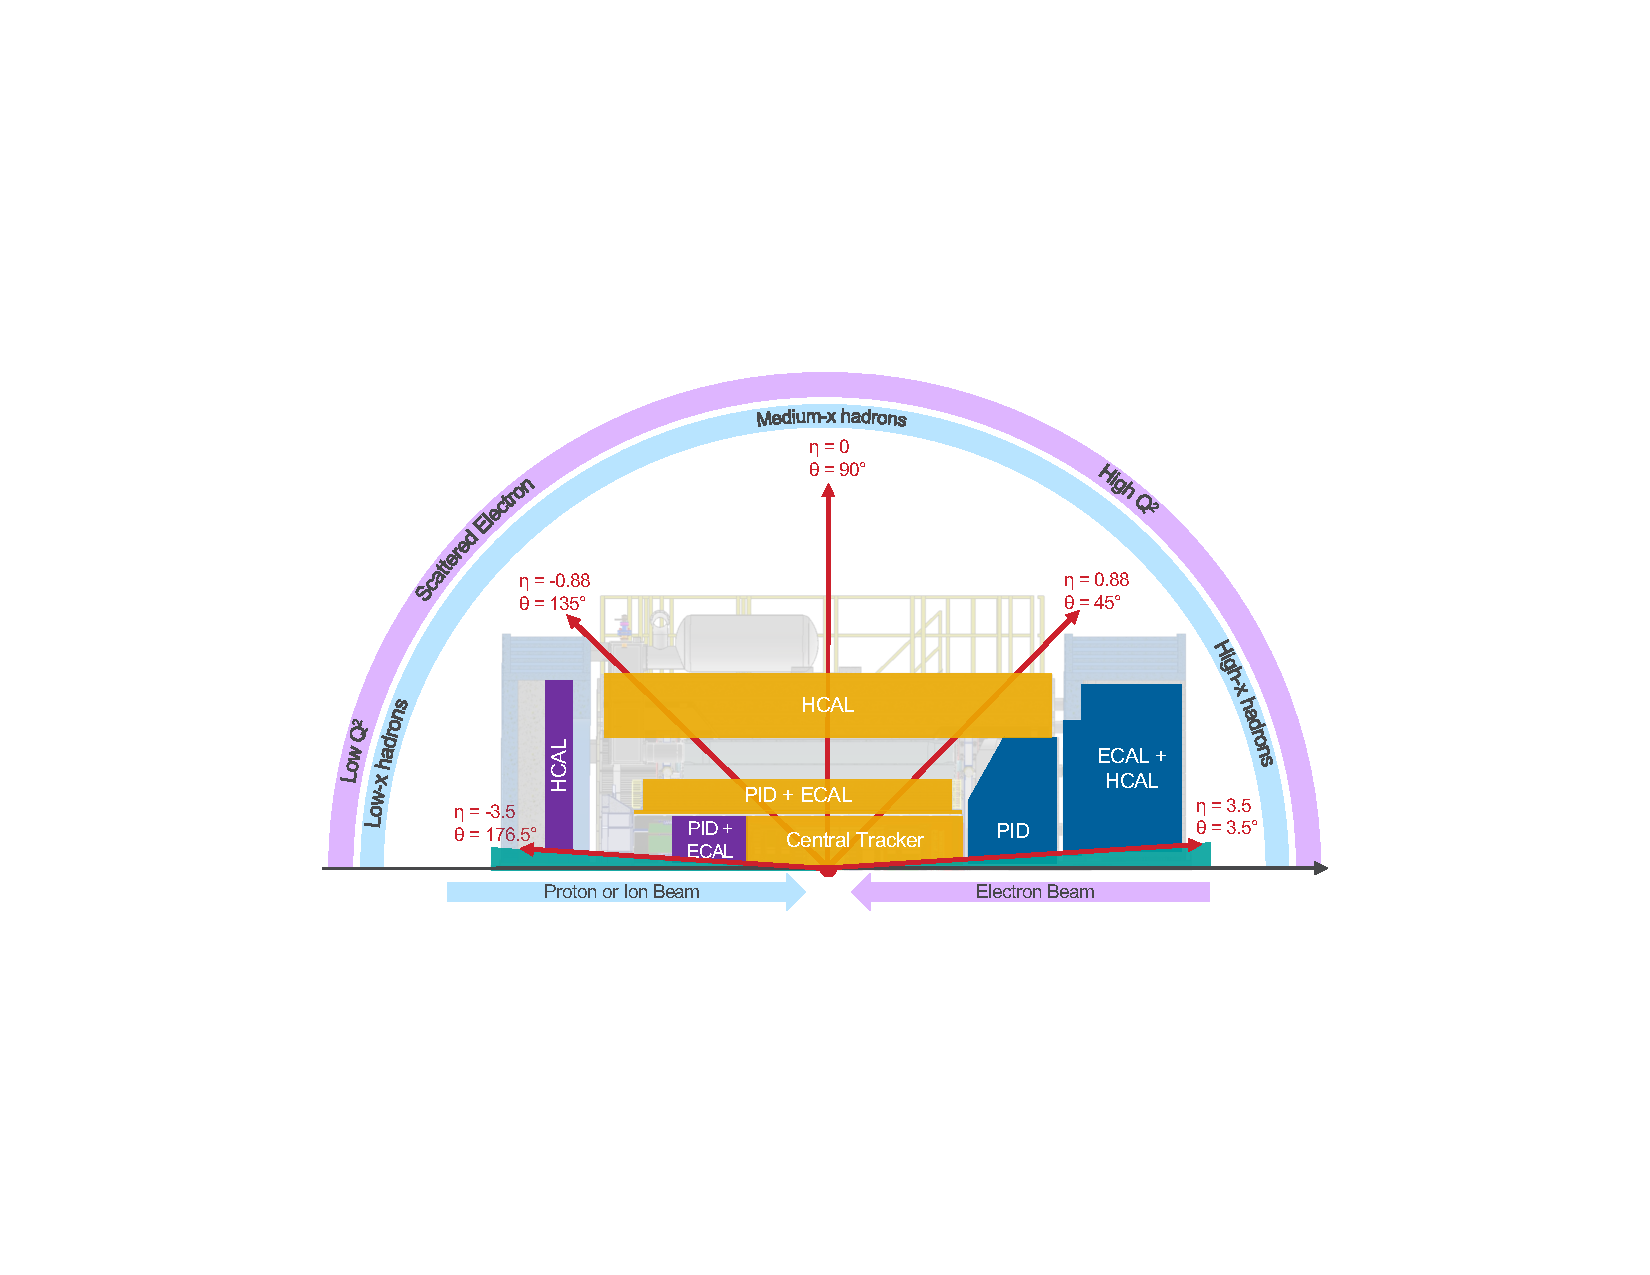
\includegraphics[width=.8\linewidth]{img/range.pdf}
%     \caption{always this image \url{https://doi.org/10.5281/zenodo.14939545}}
%     \label{fig:eic:range}
% \end{figure}